%%% AAMAS 2027 submission (main track, anonymous). Build: paper/build.sh
\documentclass[sigconf,anonymous]{aamas}

\usepackage{balance}
\usepackage{booktabs}
\usepackage{multirow}
\usepackage{amsmath}
\usepackage{xspace}
\usepackage{algorithm}
\usepackage{algorithmic}
% fonts of the template (Linux Libertine, Inconsolata) installed in the user texmf: load their maps explicitly
\pdfmapfile{+libertine.map}\pdfmapfile{+zi4.map}\pdfmapfile{+newtx.map}

%%% AAMAS-2027 copyright block (do not change!)
\makeatletter
\gdef\@copyrightpermission{
  \begin{minipage}{0.2\columnwidth}
   \href{https://creativecommons.org/licenses/by/4.0/}{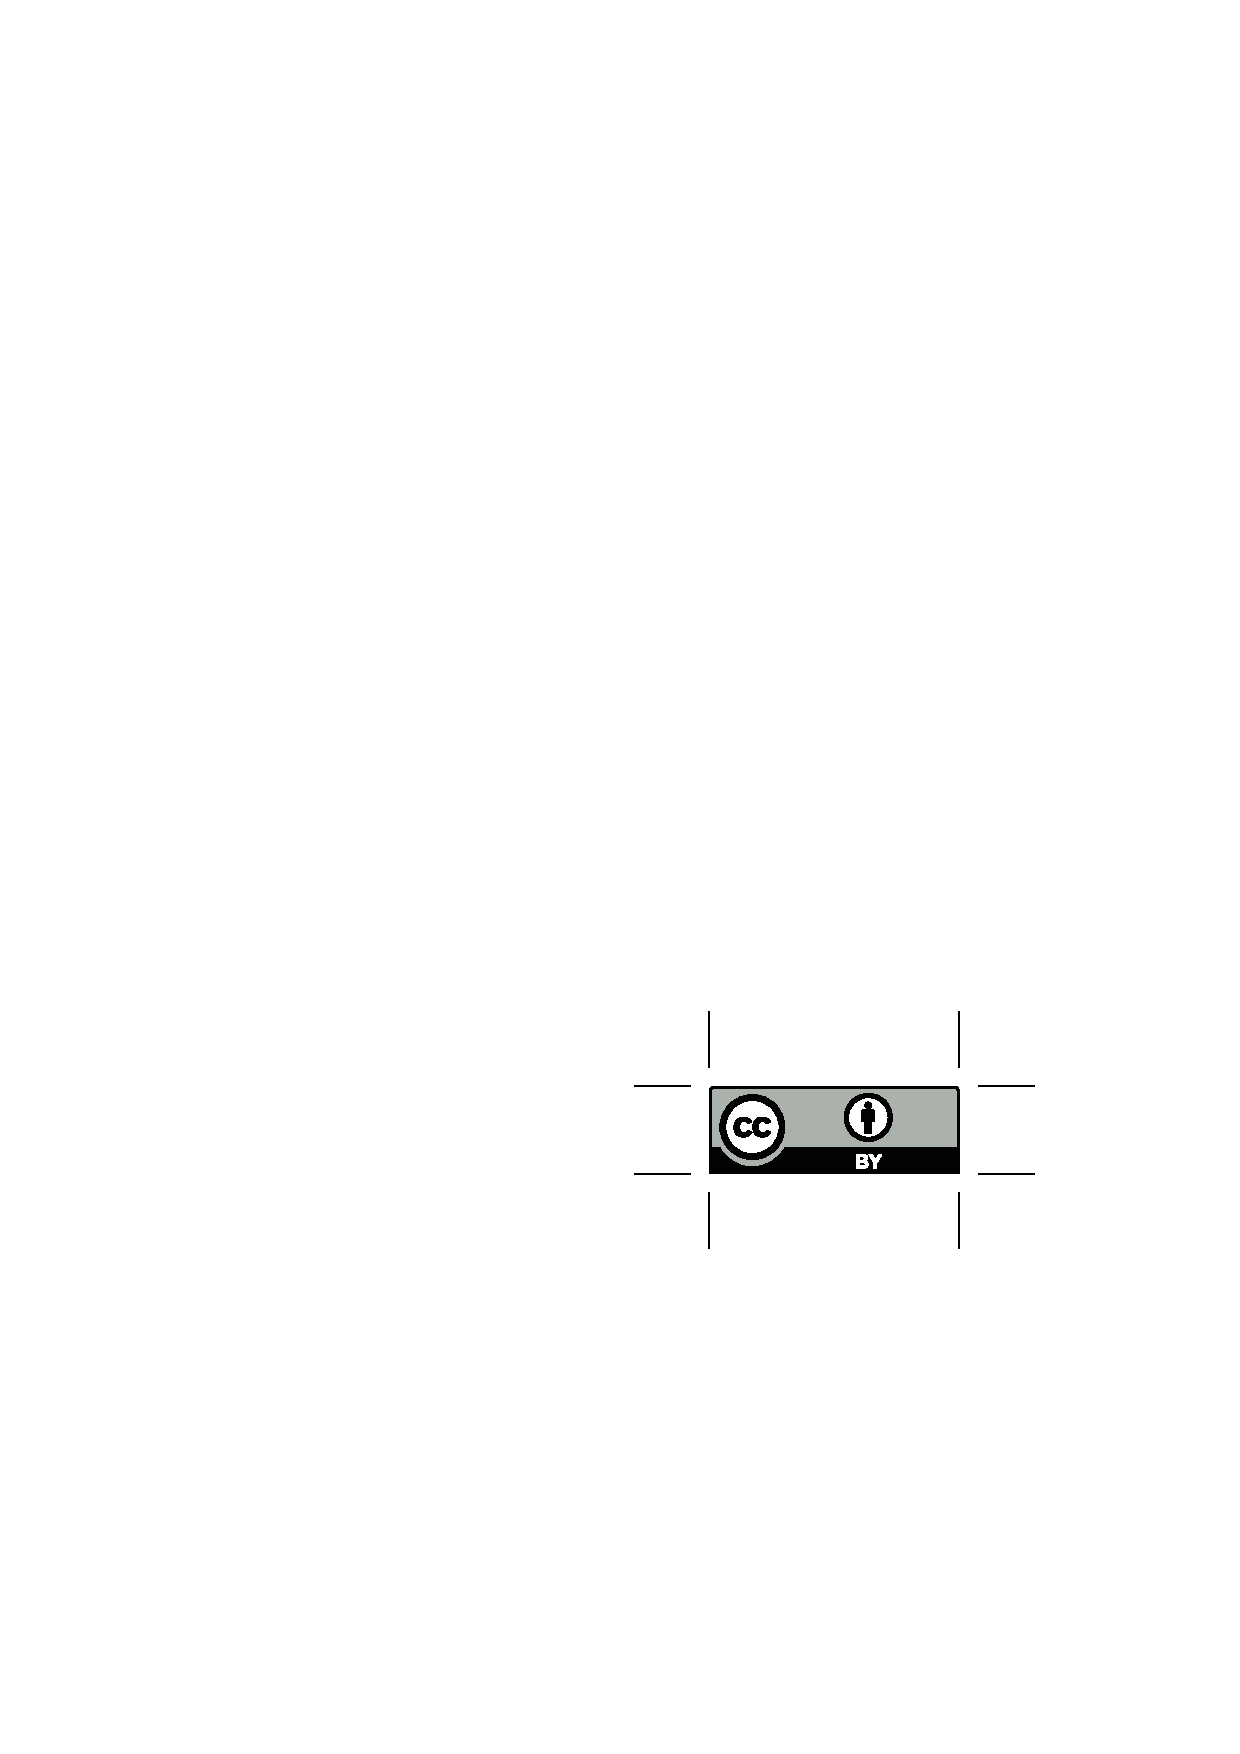
\includegraphics[width=0.90\textwidth]{by}}
  \end{minipage}\hfill
  \begin{minipage}{0.8\columnwidth}
   \href{https://creativecommons.org/licenses/by/4.0/}{This work is licensed under a Creative Commons Attribution International 4.0 License.}
  \end{minipage}
  \vspace{5pt}
}
\makeatother

\setcopyright{ifaamas}
\acmConference[AAMAS 2027]{Proc.\@ of the 26th International Conference
on Autonomous Agents and Multiagent Systems (AAMAS 2027)}{3--7 May 2027}{Hanoi, Vietnam}{M.~Baldoni, F.~Fang, W.~Yeoh, N.~Yorke-Smith (eds.)}
\copyrightyear{2027}
\acmYear{2027}
\acmDOI{}
\acmISBN{}

\acmSubmissionID{<<OpenReview submission id>>}
\submissionType{Research Paper Track}

% generated from docs/results/val-c1 and runs/anytime_c1 by paper/tools/make_tables.py
\newcommand{\ConeBcpsatlo}{0.885}
\newcommand{\ConeBcpsathi}{0.968}
\newcommand{\ConeBpcpsatlo}{0.889}
\newcommand{\ConeBpcpsathi}{0.951}
\newcommand{\ConeBcpfulllo}{0.867}
\newcommand{\ConeBcpfullhi}{0.930}
\newcommand{\ConeBctaslo}{0.127}
\newcommand{\ConeBctashi}{0.538}
\newcommand{\ConeBconstructlo}{0.885}
\newcommand{\ConeBconstructhi}{0.934}
\newcommand{\ConeBrllo}{0.680}
\newcommand{\ConeBrlhi}{0.799}
\newcommand{\ConeBclasslo}{3.2}
\newcommand{\ConeBclasshi}{13.3}
\newcommand{\ConeBrlgainlo}{20.1}
\newcommand{\ConeBrlgainhi}{32.0}
\newcommand{\ConeBheld}{8}
\newcommand{\ConeBverdict}{is met}
\newcommand{\ConeBsettings}{8}
\newcommand{\ConeBheldlist}{single-skill binary 25/5/50; single-skill binary 50/5/50; single-skill additive 50/5/50; multi-skill additive 25/5/50; multi-skill additive 50/5/50; multi-skill additive 50/5/200; multi-skill additive 150/10/500; multi-skill additive 150/5/500}
\newcommand{\ConeBfaillist}{none}
\newcommand{\ConeBtests}{46}
\newcommand{\ConeBsig}{46}
\newcommand{\ConeBmaxp}{0.013}
\newcommand{\ConeBwon}{410}
\newcommand{\ConeBpairs}{410}
\newcommand{\ConeBBcpsatlo}{--}
\newcommand{\ConeBBcpsathi}{--}
\newcommand{\ConeBBpcpsatlo}{0.907}
\newcommand{\ConeBBpcpsathi}{0.956}
\newcommand{\ConeBBcpfulllo}{0.886}
\newcommand{\ConeBBcpfullhi}{0.944}
\newcommand{\ConeBBctaslo}{--}
\newcommand{\ConeBBctashi}{--}
\newcommand{\ConeBBconstructlo}{0.899}
\newcommand{\ConeBBconstructhi}{0.943}
\newcommand{\ConeBBrllo}{--}
\newcommand{\ConeBBrlhi}{--}
\newcommand{\ConeBBclasslo}{4.4}
\newcommand{\ConeBBclasshi}{11.4}
\newcommand{\ConeBBrlgainlo}{--}
\newcommand{\ConeBBrlgainhi}{--}
\newcommand{\ConeBBheld}{6}
\newcommand{\ConeBBverdict}{is met}
\newcommand{\ConeBBsettings}{6}
\newcommand{\ConeBBheldlist}{single-skill binary 25/5/50; single-skill binary 50/5/50; single-skill additive 50/5/50; multi-skill additive 25/5/50; multi-skill additive 50/5/50; multi-skill additive 50/5/200}
\newcommand{\ConeBBfaillist}{none}
\newcommand{\ConeBBtests}{17}
\newcommand{\ConeBBsig}{17}
\newcommand{\ConeBBmaxp}{9.4e-05}
\newcommand{\ConeBBwon}{170}
\newcommand{\ConeBBpairs}{170}
\newcommand{\Ctwocpsatlo}{0.934}
\newcommand{\Ctwocpsathi}{0.995}
\newcommand{\Ctwopcpsatlo}{0.927}
\newcommand{\Ctwopcpsathi}{0.987}
\newcommand{\Ctwocpfulllo}{0.920}
\newcommand{\Ctwocpfullhi}{0.982}
\newcommand{\Ctwoctaslo}{0.133}
\newcommand{\Ctwoctashi}{0.553}
\newcommand{\Ctwoconstructlo}{0.933}
\newcommand{\Ctwoconstructhi}{0.995}
\newcommand{\Ctworllo}{0.753}
\newcommand{\Ctworlhi}{0.833}
\newcommand{\Ctwoclasslo}{0.5}
\newcommand{\Ctwoclasshi}{8.0}
\newcommand{\Ctworlgainlo}{16.7}
\newcommand{\Ctworlgainhi}{24.7}
\newcommand{\Ctwoheld}{4}
\newcommand{\Ctwoverdict}{is not met}
\newcommand{\Ctwosettings}{8}
\newcommand{\Ctwoheldlist}{single-skill binary 25/5/50; multi-skill additive 25/5/50; multi-skill additive 50/5/50; multi-skill additive 50/5/200}
\newcommand{\Ctwofaillist}{single-skill binary 50/5/50 (against CP-LNS, Parallel CP-LNS); single-skill additive 50/5/50 (against CP-LNS, Parallel CP-LNS, CP-SAT full, Greedy restarts); multi-skill additive 150/10/500 (against Greedy restarts); multi-skill additive 150/5/500 (against CP-LNS, Parallel CP-LNS)}
\newcommand{\Ctwotests}{46}
\newcommand{\Ctwosig}{37}
\newcommand{\Ctwomaxp}{0.27}
\newcommand{\Ctwowon}{395}
\newcommand{\Ctwopairs}{410}
\newcommand{\CtwoOnecpsatlo}{0.937}
\newcommand{\CtwoOnecpsathi}{1.014}
\newcommand{\CtwoOnepcpsatlo}{0.934}
\newcommand{\CtwoOnepcpsathi}{1.006}
\newcommand{\CtwoOnecpfulllo}{0.923}
\newcommand{\CtwoOnecpfullhi}{1.002}
\newcommand{\CtwoOnectaslo}{0.133}
\newcommand{\CtwoOnectashi}{0.564}
\newcommand{\CtwoOneconstructlo}{0.937}
\newcommand{\CtwoOneconstructhi}{1.014}
\newcommand{\CtwoOnerllo}{0.759}
\newcommand{\CtwoOnerlhi}{0.841}
\newcommand{\CtwoOneclasslo}{-1.4}
\newcommand{\CtwoOneclasshi}{7.7}
\newcommand{\CtwoOnerlgainlo}{15.9}
\newcommand{\CtwoOnerlgainhi}{24.1}
\newcommand{\CtwoOneheld}{3}
\newcommand{\CtwoOneverdict}{is not met}
\newcommand{\CtwoOnesettings}{8}
\newcommand{\CtwoOneheldlist}{multi-skill additive 25/5/50; multi-skill additive 50/5/50; multi-skill additive 50/5/200}
\newcommand{\CtwoOnefaillist}{single-skill binary 25/5/50 (against Parallel CP-LNS); single-skill binary 50/5/50 (against CP-LNS, Parallel CP-LNS); single-skill additive 50/5/50 (against CP-LNS, Parallel CP-LNS, CP-SAT full, Greedy restarts); multi-skill additive 150/10/500 (against CP-LNS, Parallel CP-LNS, CP-SAT full, Greedy restarts); multi-skill additive 150/5/500 (against CP-LNS, Parallel CP-LNS, CP-SAT full, Greedy restarts)}
\newcommand{\CtwoOnetests}{46}
\newcommand{\CtwoOnesig}{31}
\newcommand{\CtwoOnemaxp}{1}
\newcommand{\CtwoOnewon}{361}
\newcommand{\CtwoOnepairs}{410}
\newcommand{\CtwoHalfcpsatlo}{0.953}
\newcommand{\CtwoHalfcpsathi}{1.021}
\newcommand{\CtwoHalfpcpsatlo}{0.963}
\newcommand{\CtwoHalfpcpsathi}{1.011}
\newcommand{\CtwoHalfcpfulllo}{0.940}
\newcommand{\CtwoHalfcpfullhi}{1.007}
\newcommand{\CtwoHalfctaslo}{0.136}
\newcommand{\CtwoHalfctashi}{0.568}
\newcommand{\CtwoHalfconstructlo}{0.954}
\newcommand{\CtwoHalfconstructhi}{1.019}
\newcommand{\CtwoHalfrllo}{0.765}
\newcommand{\CtwoHalfrlhi}{0.852}
\newcommand{\CtwoHalfclasslo}{-2.1}
\newcommand{\CtwoHalfclasshi}{6.0}
\newcommand{\CtwoHalfrlgainlo}{14.8}
\newcommand{\CtwoHalfrlgainhi}{23.5}
\newcommand{\CtwoHalfheld}{1}
\newcommand{\CtwoHalfverdict}{is not met}
\newcommand{\CtwoHalfsettings}{8}
\newcommand{\CtwoHalfheldlist}{multi-skill additive 50/5/200}
\newcommand{\CtwoHalffaillist}{single-skill binary 25/5/50 (against Parallel CP-LNS); single-skill binary 50/5/50 (against CP-LNS, Parallel CP-LNS, CP-SAT full); single-skill additive 50/5/50 (against CP-LNS, Parallel CP-LNS, CP-SAT full, Greedy restarts); multi-skill additive 25/5/50 (against CP-LNS, Greedy restarts); multi-skill additive 50/5/50 (against Parallel CP-LNS, Greedy restarts); multi-skill additive 150/10/500 (against CP-LNS, Parallel CP-LNS, CP-SAT full, Greedy restarts); multi-skill additive 150/5/500 (against CP-LNS, Parallel CP-LNS, CP-SAT full, Greedy restarts)}
\newcommand{\CtwoHalftests}{46}
\newcommand{\CtwoHalfsig}{26}
\newcommand{\CtwoHalfmaxp}{1}
\newcommand{\CtwoHalfwon}{348}
\newcommand{\CtwoHalfpairs}{410}
\newcommand{\Workerslo}{0.973}
\newcommand{\Workershi}{0.996}
\newcommand{\Workersgainlo}{0.4}
\newcommand{\Workersgainhi}{2.7}
\newcommand{\Cpualnslo}{0.99}
\newcommand{\Cpualnshi}{1.00}
\newcommand{\Gapalnslo}{0.0}
\newcommand{\Gapalnshi}{1.5}
\newcommand{\Cpucpsatlo}{0.28}
\newcommand{\Cpucpsathi}{0.79}
\newcommand{\Gapcpsatlo}{3.6}
\newcommand{\Gapcpsathi}{13.3}
\newcommand{\Cpupcpsatlo}{0.99}
\newcommand{\Cpupcpsathi}{1.00}
\newcommand{\Gappcpsatlo}{5.5}
\newcommand{\Gappcpsathi}{13.5}
\newcommand{\Cpucpfulllo}{0.43}
\newcommand{\Cpucpfullhi}{0.90}
\newcommand{\Gapcpfulllo}{7.8}
\newcommand{\Gapcpfullhi}{15.8}
\newcommand{\Cpuctaslo}{0.43}
\newcommand{\Cpuctashi}{0.97}
\newcommand{\Gapctaslo}{87.3}
\newcommand{\Gapctashi}{881.6}
\newcommand{\Cpuconstructlo}{1.00}
\newcommand{\Cpuconstructhi}{1.00}
\newcommand{\Gapconstructlo}{8.1}
\newcommand{\Gapconstructhi}{14.6}
\newcommand{\Cpurllo}{0.94}
\newcommand{\Cpurlhi}{0.99}
\newcommand{\Gaprllo}{27.2}
\newcommand{\Gaprlhi}{47.1}
\newcommand{\OneCoreBoneAhead}{8}
\newcommand{\RestartsRLlo}{13}
\newcommand{\RestartsRLhi}{23}
\newcommand{\CtasSolved}{12}
\newcommand{\CtasRuns}{60}
\newcommand{\LateBone}{0}
\newcommand{\RunsBone}{480}
\newcommand{\RLNlo}{3}
\newcommand{\RLNhi}{24}
\newcommand{\ItsFiftylo}{7{,}700}
\newcommand{\ItsFiftyhi}{12{,}800}
\newcommand{\ItsFivehundred}{4{,}300}
\newcommand{\RefValFreelo}{2.8}
\newcommand{\RefValFreehi}{12.0}
\newcommand{\RefValFreematched}{0}
\newcommand{\RefValInstances}{70}
\newcommand{\RefValBoundlo}{12}
\newcommand{\RefValBoundhi}{58}
\newcommand{\RefTestFreelo}{--}
\newcommand{\RefTestFreehi}{--}
\newcommand{\RefTestFreematched}{0}
\newcommand{\RefTestInstances}{0}
\newcommand{\RefTestBoundlo}{--}
\newcommand{\RefTestBoundhi}{--}
\newcommand{\RLsamplegainlo}{--}
\newcommand{\RLsamplegainhi}{--}

% generated by paper/tools/sensitivity.py --split val
\newcommand{\LateRL}{0}
\newcommand{\LateALNS}{0}
\newcommand{\LateOther}{0}
\newcommand{\Senscpsatgainlo}{3.2}
\newcommand{\Senscpsatgainhi}{11.5}
\newcommand{\Senspcpsatgainlo}{4.9}
\newcommand{\Senspcpsatgainhi}{11.1}
\newcommand{\Senscpfullgainlo}{7.0}
\newcommand{\Senscpfullgainhi}{13.3}
\newcommand{\Sensctasgainlo}{46.2}
\newcommand{\Sensctasgainhi}{87.3}
\newcommand{\Sensconstructgainlo}{6.6}
\newcommand{\Sensconstructgainhi}{11.5}
\newcommand{\Sensrlgainlo}{20.1}
\newcommand{\Sensrlgainhi}{32.0}

\newcommand{\alns}{ALNS\xspace}
\newcommand{\Bone}{$B_1$\xspace}
\newcommand{\Btwo}{$2B_1$\xspace}

\title[ALNS for Heterogeneous Multi-Robot Coalition Scheduling]{Search Beats Learning at Equal Compute: A Pre-Registered
Study of Heterogeneous Multi-Robot Coalition Formation and Scheduling}

\author{Anonymous Author(s)}
\affiliation{\institution{Anonymous Institution}\country{Anonymous}}

\begin{abstract}
Heterogeneous robot teams must form coalitions whose combined capabilities cover each task's requirements and
whose members arrive together before the task can start. This couples coalition formation, routing and scheduling,
and learned policies have recently been reported as the state of the art for it. We ask whether that claim survives a
comparison at equal compute. We present an adaptive large neighbourhood search (ALNS) over a deadlock-free plan
representation, a global task order with a minimal covering coalition per task, whose evaluator reproduces the
benchmark's simulator exactly and scores an insertion move in time linear in the coalition size. On the HeteroMRTA
benchmark, with up to 150 robots and 500 tasks, we compare it with the published reinforcement-learning policy,
three methods built on the constraint solver CP-SAT (including a fully parallel large neighbourhood search), the exact
MILP the benchmark used (CTAS-D, ported to an open solver and checked against the original authors' solutions), and
greedy restarts.
All methods run on the same pinned cores at the benchmark's own time budgets, and the confirmatory test run follows a
pre-registration frozen before it. ALNS is significantly better than every competitor on \ConeBheld{} of the 8
settings: its plans are \mbox{\ConeBclasslo--\ConeBclasshi\%} shorter than those of the CP-SAT-based methods and
greedy restarts, and \mbox{\ConeBrlgainlo--\ConeBrlgainhi\%} shorter than those of the learned policy, which runs at its
published time budget on the same CPUs. Making CP-SAT fully parallel does not close the gap, and the exact MILP finds a plan within the budget
for only \CtasSolved{} of the \CtasRuns{} instances with up to 200 tasks. On one core and in 2\,s, ALNS is already significantly better than every eight-core competitor on
\Ctwoheld{} of the 8 settings.

\end{abstract}

\keywords{Multi-robot task allocation; Coalition formation; Scheduling with synchronization; Large neighbourhood
search; Constraint programming; Benchmarking}

\begin{document}

\pagestyle{fancy}
\fancyhead{}

\maketitle

\section{Introduction}
\label{sec:intro}

\begin{figure*}[t]
\centering
\resizebox{\textwidth}{!}{% Overview figure (TikZ). Included by main.tex; needs tikz with the libraries arrows.meta, calc, patterns and
% decorations.pathreplacing. Colours: Okabe-Ito (colour-blind safe), as in the data figures.
\definecolor{oiBlue}{HTML}{0072B2}\definecolor{oiOrange}{HTML}{E69F00}\definecolor{oiVerm}{HTML}{D55E00}
\definecolor{oiGreen}{HTML}{009E73}\definecolor{oiPink}{HTML}{CC79A7}
\begin{tikzpicture}[
    x=1cm, y=1cm, font=\scriptsize, >={Stealth[length=1.6mm]},
    panel/.style={draw=#1, line width=0.6pt, rounded corners=2pt},
    head/.style={fill=#1, text=white, font=\footnotesize\bfseries, anchor=north west, inner sep=2pt,
                 minimum height=3.6mm, rounded corners=1pt},
    robot/.style={circle, fill=#1, draw=black!70, line width=0.3pt, minimum size=2.4mm, inner sep=0pt},
    task/.style={circle, draw=black!80, fill=white, line width=0.5pt, minimum size=4.2mm, inner sep=0pt,
                 font=\tiny\bfseries},
    depot/.style={rectangle, fill=#1, draw=black!70, line width=0.3pt, minimum size=2.4mm, inner sep=0pt},
    tbox/.style={rectangle, rounded corners=1pt, draw=black!70, fill=black!4, minimum width=6.2mm,
                 minimum height=4.2mm, inner sep=1pt, font=\tiny\bfseries},
    step/.style={rectangle, rounded corners=4pt, draw=#1, fill=#1!12, line width=0.5pt, align=center,
                 inner sep=1.2pt, font=\tiny, text width=10.5mm, minimum height=6.2mm},
    meth/.style={rectangle, rounded corners=1pt, draw=black!50, fill=black!3, inner sep=1pt,
                 minimum width=21mm, minimum height=3.1mm, font=\tiny, anchor=west},
    chev/.style={rectangle, rounded corners=1pt, draw=#1, fill=#1!12, font=\tiny, align=center, inner sep=1.2pt,
                 minimum height=6.5mm, text width=9.2mm},
    note/.style={font=\tiny, align=left, anchor=west, execute at begin node={\hyphenpenalty=10000}},
  ]
% ---------------------------------------------------------------------------------------------------------------
% (a) Problem
\draw[panel=oiBlue] (0,0) rectangle (5.25,5.3);
\node[head=oiBlue] at (0.05,5.25) {(a) Coalitions with synchronised starts};
\node[depot=oiBlue] (dA) at (0.4,4.35) {};
\node[robot=oiBlue] (r1) at (0.95,4.35) {};
\node[anchor=south west, font=\tiny, text=oiBlue, inner sep=1pt] at ([xshift=-1.5mm]r1.north) {traits $a_1{=}(1,0,1)$};
\node[depot=oiOrange] (dB) at (0.4,2.7) {};
\node[robot=oiOrange] (r2) at (0.95,2.7) {};
\node[anchor=north west, font=\tiny, text=oiOrange!80!black, inner sep=1pt] at ([xshift=-1.5mm]r2.south)
  {traits $a_2{=}(0,1,1)$};
\node[task] (t1) at (2.75,3.5) {1};
\node[note, align=left] at ([xshift=0.4mm]t1.east) {needs\\$r_1{=}(1,1,0)$};
\node[task] (t2) at (4.7,4.5) {2};
\node[task] (t3) at (4.7,2.55) {3};
\draw[->, dashed, oiBlue, line width=0.5pt] (r1) to[bend left=10] (t1);
\draw[->, dashed, oiOrange!85!black, line width=0.5pt] (r2) to[bend right=10] (t1);
\draw[->, dashed, oiBlue, line width=0.5pt] (t1) to[bend left=12] (t2);
\draw[->, dashed, oiOrange!85!black, line width=0.5pt] (t1) to[bend right=12] (t3);
\node[depot=black!45] at (0.35,2.05) {};
\node[note] at (0.45,2.05) {depot};
\node[robot=black!45] at (1.25,2.05) {};
\node[note] at (1.35,2.05) {robot};
\node[task, minimum size=2.4mm] at (2.1,2.05) {};
\node[note] at (2.2,2.05) {task};
\node[note] at (2.9,2.05) {goal: min.\ makespan};
% timeline of task 1
\draw[->, black!70] (0.35,0.45) -- (5.1,0.45) node[anchor=north east, font=\tiny] {time};
\node[anchor=east, font=\tiny, text=oiBlue] at (0.98,1.38) {robot 1};
\node[anchor=east, font=\tiny, text=oiOrange!80!black] at (0.98,0.88) {robot 2};
\draw[oiBlue, line width=0.5pt] (1.0,1.38) -- (1.7,1.38);
\fill[oiBlue] (1.7,1.38) circle (0.6mm);
\fill[pattern=north east lines, pattern color=oiBlue!70] (1.7,1.28) rectangle (2.75,1.48);
\node[anchor=south, font=\tiny] at (2.22,1.48) {arrives, waits};
\draw[oiOrange, line width=0.5pt] (1.0,0.88) -- (2.75,0.88);
\fill[oiOrange] (2.75,0.88) circle (0.6mm);
\fill[oiGreen!55] (2.75,0.78) rectangle (3.85,1.48);
\node[font=\tiny, align=center] at (3.3,1.13) {task 1\\together};
\draw[densely dotted] (2.75,0.45) -- (2.75,1.62);
\draw[densely dotted] (3.85,0.45) -- (3.85,1.62);
\node[anchor=north, font=\tiny] at (2.75,0.45) {$s_1$};
\node[anchor=north, font=\tiny] at (3.85,0.45) {$f_1{=}s_1{+}d_1$};
\node[note] at (3.92,1.13) {on to 2, 3};
% ---------------------------------------------------------------------------------------------------------------
% (b) Method
\draw[panel=oiVerm] (5.45,0) rectangle (11.85,5.3);
\node[head=oiVerm] at (5.5,5.25) {(b) ALNS over a deadlock-free plan};
\node[note] at (5.55,4.68) {plan: a global task order $\pi$ and a minimal cover $C_j$ per task};
\node[tbox] (p1) at (6.0,4.12) {1};
\node[tbox] (p2) at (7.0,4.12) {3};
\node[tbox] (p3) at (8.0,4.12) {2};
\node[tbox] (p4) at (9.0,4.12) {$\cdots$};
\draw[->] (p1) -- (p2); \draw[->] (p2) -- (p3); \draw[->] (p3) -- (p4);
\node[robot=oiBlue, minimum size=1.8mm] at ([yshift=-3.3mm, xshift=-1.2mm]p1.south) {};
\node[robot=oiOrange, minimum size=1.8mm] at ([yshift=-3.3mm, xshift=1.2mm]p1.south) {};
\node[robot=oiOrange, minimum size=1.8mm] at ([yshift=-3.3mm]p2.south) {};
\node[robot=oiBlue, minimum size=1.8mm] at ([yshift=-3.3mm]p3.south) {};
\node[note, text width=22mm] at (9.45,4.0) {robots visit their tasks in the order $\pi$: no deadlock; forward pass = simulator};
% ALNS loop
\coordinate (c) at (7.05,1.95);
\node[step=oiBlue] (d) at ($(c)+(0,0.95)$) {destroy\\$q$ tasks};
\node[step=oiOrange] (r) at ($(c)+(1.0,0)$) {exact\\repair};
\node[step=oiPink] (a) at ($(c)+(0,-0.95)$) {accept by\\annealing};
\node[step=oiGreen] (w) at ($(c)+(-1.0,0)$) {adapt\\weights};
\draw[->, line width=0.6pt] (d.east) to[bend left=35] (r.north);
\draw[->, line width=0.6pt] (r.south) to[bend left=35] (a.east);
\draw[->, line width=0.6pt] (a.west) to[bend left=35] (w.south);
\draw[->, line width=0.6pt] (w.north) to[bend left=35] (d.west);
\node[font=\footnotesize\bfseries] at (c) {ALNS};
\node[font=\tiny] at (7.05,0.22) {$\times 8$ workers share their best plan every 1\,s};
% exact insertion inset
\draw[rounded corners=2pt, draw=black!60, fill=black!3] (8.7,0.15) rectangle (11.75,3.35);
\node[anchor=north west, font=\tiny\bfseries] at (8.75,3.32) {exact insertion of task $j$ in $O(|C_j|)$};
\node[tbox, minimum width=4.5mm] (q1) at (9.15,2.45) {$p$};
\node[tbox, minimum width=4.5mm, draw=oiOrange, fill=oiOrange!15] (qj) at (10.0,2.45) {$j$};
\node[tbox, minimum width=4.5mm] (qk) at (10.85,2.45) {$k_i$};
\draw[->] (q1) -- (qj); \draw[->] (qj) -- (qk);
\draw[->, black!45, densely dashed] (q1.north) to[bend left=28] (qk.north);
\draw[decorate, decoration={brace, amplitude=2pt, mirror}] ([yshift=-1mm]qk.south west) --
  ([yshift=-1mm, xshift=5mm]qk.south east) node[midway, below=1pt, font=\tiny] {tail $\theta_{k_i}$};
\node[note, text width=29mm] at (8.8,1.62) {new makespan, exactly:};
\node[note] at (8.8,1.18) {$M' = \max\!\big(M,\; s_j + d_j$\\[0.3ex]
  $\qquad + \max_{i \in C_j} (\tau_{j k_i} + \theta_{k_i})\big)$};
\node[note, text width=29mm] at (8.8,0.5) {scores every position without a forward pass; dashed: the arc that $p \to j \to k_i$ replaces};
% ---------------------------------------------------------------------------------------------------------------
% (c) Protocol
\draw[panel=oiGreen] (12.05,0) rectangle (17.6,5.3);
\node[head=oiGreen] at (12.1,5.25) {(c) Equal compute, pre-registered};
\node[chev=oiBlue] (s1) at (12.68,4.4) {dev:\\tune all};
\node[chev=oiOrange] (s2) at (13.98,4.4) {val:\\dry run};
\node[chev=oiGreen] (s3) at (15.28,4.4) {freeze\\(git trees)};
\node[chev=oiPink] (s4) at (16.58,4.4) {test:\\one run};
\draw[->] (s1) -- (s2); \draw[->] (s2) -- (s3); \draw[->] (s3) -- (s4);
\node[meth, draw=oiBlue, fill=oiBlue!12, line width=0.5pt] (m1) at (12.2,3.35) {\textbf{ALNS (ours)}};
\foreach \m [count=\i from 2] in {RL(s.$N$) policy, CP-SAT LNS, parallel CP-SAT LNS, CP-SAT model, CTAS-D (MILP),
                                 constructor restarts} {
  \node[meth] (m\i) at (12.2,3.72-0.37*\i) {\m};
}
\draw[decorate, decoration={brace, amplitude=3pt}] ([xshift=1mm]m1.north east) -- ([xshift=1mm]m7.south east)
  node[midway, right=3pt, font=\tiny, align=left] {same 8 pinned\\cores and\\budget $B_1$;\\CPU use\\recorded};
\node[rectangle, rounded corners=1pt, draw=black!60, fill=black!4, font=\tiny, align=center, text width=50mm,
      inner sep=1.5pt] (sim) at (14.82,0.45)
  {every plan scored by the benchmark's simulator;\\paired ratios, bootstrap CIs, Holm-corrected tests};
\draw[->] ([yshift=-0.5mm]m7.south) -- (m7.south |- sim.north);
\end{tikzpicture}
}
\caption{Overview. (a) Robots with binary trait vectors must gather in coalitions that cover each task's requirement
vector; a task starts when its last member arrives, so a late member delays the whole coalition and everything after
it. (b) Our ALNS searches over a global task order with a minimal covering coalition per task, which cannot deadlock
and is evaluated exactly; insertions are scored in time linear in the coalition size from longest-path tails
(Eq.~\eqref{eq:insert}). (c) Every method runs on the same pinned cores for the same budget, under a pre-registration
frozen before the single run on the test split.}
\label{fig:overview}
\end{figure*}

Teams of heterogeneous robots are deployed for search and rescue, inspection and construction, where many tasks need
capabilities that no single robot has \cite{kashino2020aerial,korsah2013comprehensive}. A task can then only start
once a coalition whose combined capabilities cover its requirements has gathered at its location, and every member
waits for the last one to arrive. Allocating coalitions, ordering each robot's tasks and timing the joint starts are
therefore one coupled problem: a robot that arrives late delays every task downstream of its coalition partners, and
an inconsistent ordering of shared tasks can deadlock the team. Such problems, where the schedules of different robots
constrain each other, are the hardest classes of the multi-robot task allocation taxonomies
\cite{gerkey2004formal,korsah2013comprehensive}.

Recent work has approached this problem with learned policies. \citet{dai2025heterogeneous} train a decentralised
policy by reinforcement learning (RL), with which each robot chooses its next task through an attention mechanism,
and report that it closely matches or outperforms heuristic and mixed-integer programming baselines while being at
least two orders of magnitude faster. Their best variant samples ten rollouts, RL(s.10), and scales to 150 robots and
500 tasks on the HeteroMRTA benchmark that they release, while the exact baseline, the MILP CTAS-D
\cite{fu2023robust}, solves few instances of most 50-task settings within an hour. Related learned approaches form
coalitions and routes for homogeneous teams \cite{dai2024dynamic} or schedule heterogeneous coalitions with precedence
constraints by imitation learning \cite{bichler2025sadcher}. In the HeteroMRTA evaluation, the classical competitors
are an exact solver stopped at a time limit, ant colony heuristics \cite{babincsak2023ant} and a greedy rule, and
each method runs at its own time budget.

Operations research has a long record of strong anytime heuristics for closely related problems, in particular
large neighbourhood search (LNS) for vehicle routing with synchronisation constraints
\cite{drexl2012synchronization,hojabri2018large,parragh2018solving}. It is therefore natural to ask how much of the
reported advantage of learned policies survives a comparison with a well-engineered search method and strong
constraint-programming baselines, when every method gets the same wall-clock time on the same cores. We answer this
question on HeteroMRTA with a pre-registered, compute-matched study (Figure~\ref{fig:overview}).

\paragraph{Contributions.}
\begin{itemize}
\item \textbf{An ALNS for coalition formation and scheduling with synchronisation} (Section~\ref{sec:method}). Plans
  are a global task order with one minimal covering coalition per task. This representation is deadlock-free by
  construction, its forward pass reproduces the benchmark's own simulator bit for bit, and an insertion move is
  evaluated exactly in time linear in the coalition size from longest-path tails.
\item \textbf{A compute-matched evaluation protocol} (Section~\ref{sec:setup}). All methods run in the same lanes of
  pinned physical cores at the benchmark's own budgets, with their CPU use recorded and host throttling monitored.
  Competitors are tuned on a separate split. The hypotheses, competitors, budgets and analysis were frozen, and the
  frozen code identified by its git trees, before the single run on the test split.
\item \textbf{Strong competitors.} Besides the published RL policy and constructor restarts, we compare with
  CP-SAT LNS in a threaded and a properly parallel form, with CP-SAT's own portfolio on the full model, and with
  CTAS-D, which we port to an open solver and check against the benchmark authors' own Gurobi solutions.
\item \textbf{Findings} (Section~\ref{sec:results}). ALNS is significantly better than every competitor on
  \ConeBheld{} of the 8 settings with 50 to 500 tasks, with plans \ConeBclasslo--\ConeBclasshi\% shorter than
  those of the classical baselines and \ConeBrlgainlo--\ConeBrlgainhi\% shorter than those of the learned policy.
  Parallelising CP-SAT does not close the gap, the exact MILP rarely produces a plan within the budget, and ALNS on a
  single core for 2\,s is already significantly better than every eight-core competitor at the full budget on
  \Ctwoheld{} of the 8 settings.
\end{itemize}

We take no position against learning for multi-robot coordination. Our results say that on this benchmark, at equal
compute, careful search is the stronger method, and that learned planners should be evaluated against such search
at matched budgets. The code and every result row are provided with the paper.

\section{Problem}
\label{sec:problem}

We use the problem and the benchmark of \citet{dai2025heterogeneous} unchanged. An instance has agents
$A = \{1, \dots, n\}$, tasks $T = \{1, \dots, m\}$ and $K$ traits. Agent $i$ has a binary trait vector
$a_i \in \{0, 1\}^K$ shared by all agents of its species, starts and ends at its species' depot $o_i$ and moves at a
common speed $v$. Task $j$ has a location $x_j$, a duration $d_j$ and a requirement vector $r_j \in \mathbb{N}^K$. Travel
times are Euclidean, $\tau_{jk} = \lVert x_j - x_k \rVert / v$ between tasks and $\tau^0_{ij} = \lVert o_i - x_j \rVert
/ v$ between agent $i$'s depot and task $j$.

A plan gives every task $j$ a coalition $C_j \subseteq A$ whose traits cover its requirement,
$\sum_{i \in C_j} a_i \ge r_j$ componentwise,
and every agent a route, the sequence of the tasks whose coalitions it belongs to. Agents leave their depots at time 0.
Task $j$ starts when the last member arrives, $s_j = \max_{i \in C_j} \alpha_{ij}$, where $\alpha_{ij}$ is the arrival
time of member $i$, and it occupies all members until $f_j = s_j + d_j$. A member then travels to the next task on its
route: if that task is $k$, $\alpha_{ik} = f_j + \tau_{jk}$, and after its last task it returns to its depot. The
makespan is the latest return to a depot, and the objective is to minimise it. Routes can deadlock: if one agent must
do $j$ before $k$ and another $k$ before $j$, neither task ever starts. The benchmark's simulator lets an agent join a
task only while the task is not yet covered, and it stops at simulated time 200; a plan that has not finished all
tasks by then is a failure.

In the taxonomy of \citet{gerkey2004formal} this is a single-task robot, multi-robot task problem with time-extended
assignment (ST-MR-TA): coalition formation, routing and scheduling in one. The synchronised starts are what makes it
hard for construction heuristics and for policies that choose one task at a time: a coalition's start waits for its
latest member, and that delay propagates along the routes of all members.

\paragraph{Benchmark.} HeteroMRTA \cite{dai2025heterogeneous} draws tasks and depots uniformly in the unit square,
durations uniformly in $[0, 5)$ and uses $v = 0.2$. It has three families. In SA-BT the agents are single-skilled (one
trait per species) and requirements are binary; SA-AT has additive requirements of up to two units per trait, so a
task can need two agents of one species; in MA-AT each species has a distinct random binary trait vector, so agents can have several skills.
We name a setting by its family and its numbers of robots and tasks, e.g.\ multi-skill robots with additive needs,
150 robots and 500 tasks; all settings have 5 species except one with 10. We generate
instances with the benchmark's own generator from fixed seeds, for three disjoint splits (Section~\ref{sec:setup}),
and use its simulator to score every plan.

\section{Adaptive Large Neighbourhood Search}
\label{sec:method}

Our method is an adaptive large neighbourhood search (ALNS) \cite{shaw1998using,ropke2006adaptive,pisinger2010large}:
it repeatedly removes a few tasks from the current plan and reinserts them, and it accepts the result by simulated
annealing \cite{kirkpatrick1983optimization}. Its strength comes from a plan representation in which every move is
feasible and cheap to evaluate exactly.

\subsection{Plan representation}
\label{sec:repr}

A plan is a pair $(\pi, C)$ of a global order $\pi$ of the tasks and a coalition $C_j$ for every task; every agent
visits its tasks in the order of $\pi$. A forward pass over $\pi$ computes the schedule in time
$O(\sum_j |C_j|)$: for the next task $j$, each member's arrival follows from its previous task, $s_j$ is their
maximum and $f_j = s_j + d_j$. The representation has three properties.
\begin{enumerate}
\item \emph{Deadlock-free.} Every precedence between two tasks on a route follows $\pi$, so no cycle can form.
\item \emph{Exact.} We compute travel times exactly as the benchmark's simulator does, so the forward pass reproduces
  the simulator's makespan bit for bit; our tests check this by replaying plans in the simulator, and every reported
  result is the simulator's own score.
\item \emph{Minimal covers.} Since the simulator does not let an agent join a task that is already covered, every
  $C_j$ must be a minimal cover: no member can be left out without breaking coverage. The search keeps this invariant.
\end{enumerate}
Restricting the search to such plans loses nothing:
\begin{proposition}
For every deadlock-free plan there is a plan $(\pi, C)$ with minimal covers whose makespan is not larger.
\end{proposition}
\begin{proof}[Proof sketch]
Let $\pi$ order the tasks by start time, breaking ties by a topological order of the route precedences (which exists
because the plan does not deadlock); every route follows $\pi$, and the forward pass gives the same schedule. Now drop
redundant members one at a time. Task $j$ then starts at the maximum of fewer arrivals, so not later. The dropped
member $i$ goes straight from its previous location $p$ to its next task $k$; it used to arrive at $k$ at
$f_j + \tau_{jk} \ge \alpha_{ij} + \tau_{jk} = f_p + \tau_{pj} + \tau_{jk} \ge f_p + \tau_{pk}$ by the triangle
inequality, so it arrives no later. Since starts are monotone in arrivals, no task starts later and no agent returns
later.
\end{proof}

\subsection{Exact insertion in linear time}
\label{sec:insertion}

The central operation inserts a task $j$ into a plan that lacks it: it chooses a position in $\pi$ and a coalition.
Let the position be after the prefix $\pi_{1..p}$. The prefix schedule does not change, so the arrival of every agent
at $j$ is known. We take the \emph{earliest-arrival cover}: add agents that contribute to an unmet requirement in
order of arrival until $j$ is covered, then drop redundant members, latest arrival first. This is a minimal cover
with the earliest possible start $s_j$ at that position.

The new makespan follows in $O(|C_j|)$. The earliest-start schedule is a longest-path computation in the acyclic graph
of the routes, so let the \emph{tail} $\theta_k$ of a task be the length of the longest path from its start to the
end: $\theta_k = d_k$ plus the largest, over its members, of the travel to that member's next task plus that task's
tail, or of the travel home. Inserting $j$ adds paths through $j$ and replaces each member's route arc $p \to k$ by
$p \to j \to k$, which is never shorter by the triangle inequality. Hence the makespan after the insertion is exactly
\begin{equation}
  M' = \max\Big(M,\; s_j + d_j + \max_{i \in C_j} \big(\tau_{j k_i} + \theta_{k_i}\big)\Big),
  \label{eq:insert}
\end{equation}
where $M$ is the old makespan, $k_i$ is member $i$'s next task after the position ($\tau_{jk_i} + \theta_{k_i}$ is
replaced by the travel home if there is none), and the tails are those of the old plan, since no task after the
position has a path to $j$. One sweep over $\pi$ updates the agents' arrivals at $j$ incrementally and scores every
position; positions where no capable agent's arrival changed are skipped, and for plans with more than 64 positions
only 64 are tried: the first, the last and those next to $j$'s nearest tasks.

The search objective is the makespan plus $\lambda$ times the mean finish time ($\lambda = 0.1$), which breaks the
many ties in makespan and rewards schedules with slack. For the second term, the delays that the new coalition causes
at its members' next tasks give a lower bound for every position; positions are then evaluated best-first by this
bound, with a forward pass that re-runs only agents whose state differs from the old schedule and stops as soon as
none does, until the bound exceeds the best position found. The chosen insertion is thus exact, and the whole
evaluation is identical to a full forward pass (which our tests check).

\subsection{Search}
\label{sec:search}

\begin{algorithm}[t]
\caption{ALNS worker (one process)}
\label{alg:alns}
\begin{algorithmic}[1]
\STATE $x \gets$ best of randomized constructions, run for 5\% of the budget
\STATE $x^* \gets x$; operator weights $w \gets 1$; temperature $t \gets t_0$
\WHILE{time remains}
  \STATE pick destroy $D$ and repair $R$ by roulette on $w$; $q \sim U\{1, \dots, q_{\max}\}$
  \STATE $x' \gets R(D(x, q))$ \COMMENT{or exchange of route tails}
  \IF{$g(x') \le g(x)$ or $u < e^{-(g(x') - g(x))/t}$}
    \STATE $x \gets x'$; with probability 0.1 re-sort $\pi$ by start time
    \IF{$x$ is better than $x^*$ (makespan, then $g$)} \STATE $x^* \gets x$ \ENDIF
  \ENDIF
  \STATE update scores; every 100 iterations update $w$; cool $t$
  \STATE after 3000 iterations without a new best: $x \gets x^*$
  \STATE every second: exchange $x^*$ with the other workers
\ENDWHILE
\RETURN $x^*$
\end{algorithmic}
\end{algorithm}

Algorithm~\ref{alg:alns} shows one worker; $g$ is the search objective.

\paragraph{Construction.} For the first 5\% of the budget, a worker builds plans by list scheduling
\cite{kolisch1996serial} (repeatedly append the task whose earliest-arrival cover starts first), by the same with noisy scores, and, up to 100 tasks, by
random-order best insertion, and keeps the best.

\paragraph{Destroy operators} remove $q$ tasks, with $q$ uniform in $\{1, \dots, q_{\max}\}$ and
$q_{\max} = \mathrm{clip}(\mathrm{round}(4\sqrt{50/m}), 2, 6)$: large instances are short of iterations and gain from
many small moves. \emph{Random} removes uniformly; \emph{related} removes tasks close to a random seed task in a random
mix of distance, start time and requirement \cite{shaw1998using}; \emph{worst wait} prefers tasks whose members wait
longest; \emph{critical} removes tasks of the chain that determines the makespan (following the latest-arriving member
back to its depot) and their spatial neighbours; \emph{route segment} removes consecutive tasks of one agent's route,
half of the time the agent that returns last. Selection is randomised by rank as in \citet{ropke2006adaptive}. A sixth
move exchanges the route tails of two agents with identical traits after a random position in $\pi$; it keeps all
covers minimal and needs no repair.

\paragraph{Repair operators} reinsert the removed tasks one at a time with the exact insertion of
Section~\ref{sec:insertion}: in random order, in random order with arrival times perturbed by up to 20\% when
choosing covers, largest requirement first, or by regret-2 (for up to ten removed tasks, else in random order).

\paragraph{Acceptance and adaptation.} Candidates are accepted by simulated annealing on $g$, with the temperature
cooled geometrically over the wall-clock budget from $t_0 = 0.01\, g_0 \min(1, (50/m)^{1.5})$ to $t_0 / 50$, where
$g_0$ is the objective of the construction. Operator weights adapt by segment scores \cite{ropke2006adaptive}. After
an accepted move the order $\pi$ is re-sorted by start time with probability 0.1; this is the same plan and schedule,
but later insertions then see positions on a time line. After 3000 iterations without a new best plan, the search
returns to the best plan.

\paragraph{Parallel workers.} On $c$ cores, $c$ independent workers with different seeds exchange their best plans
through shared memory every second: a worker publishes its best plan if it beats the shared one and adopts the shared
plan if it is strictly better. The kernels are compiled with Numba; a worker runs \ItsFiftylo--\ItsFiftyhi{} iterations per
second on the 50-task instances and about \ItsFivehundred{} on the 500-task ones. All parameters were set on a separate tuning split
(Section~\ref{sec:setup}); several other components (elite pools with crossover, kicks, growing removal sizes, member
swaps, delay-aware covers) were tried there and not kept.

\section{Related Work}
\label{sec:related}

\paragraph{Task allocation with coalitions.} Multi-robot task allocation has been classified by whether robots do
one or several tasks at a time, whether tasks need one or several robots, and whether assignments extend over time
\cite{gerkey2004formal}, and by the dependencies between schedules \cite{korsah2013comprehensive}. Coalition formation
for tasks that one agent cannot do alone goes back to \citet{shehory1998methods}; anytime coalition formation with
spatial and temporal constraints is studied by \citet{capezzuto2020anytime}. Market-based methods such as CBBA
\cite{choi2009consensus} allocate tasks to single robots in a decentralised way. Trait-based approaches allocate
coalitions by capability requirements and interleave allocation, scheduling and motion planning
\cite{neville2021interleaved,neville2023ditags}. For the heterogeneous coalition problem studied here, CTAS-D
\cite{fu2023robust} formulates a mixed-integer program over species-level flows with synchronised start times, and ant
colony optimisation has been applied to multi-skilled coalitions \cite{babincsak2023ant}.

\paragraph{Learned policies.} \citet{dai2024dynamic} learn to form coalitions and routes with an attention-based policy
trained by RL, and \citet{dai2025heterogeneous} extend this to heterogeneous agents with trait vectors and release
the HeteroMRTA benchmark that we use. \citet{bichler2025sadcher} learn by imitation to schedule heterogeneous
coalitions with precedence constraints in real time. The RL policies decide sequentially and improve by sampling rollouts, like
attention models for vehicle routing \cite{kool2019attention,kwon2020pomo}. For routing, a systematic evaluation on the
travelling salesman problem found learned solvers still behind traditional solvers in nearly all respects
\cite{liu2023how}, and \citet{accorsi2022guidelines} propose guidelines for testing learned routing methods to the
standards of operations research. On HeteroMRTA, the comparison was with an exact solver under a time limit, ant
colony heuristics and a greedy rule.

\paragraph{Routing with synchronisation.} Vehicle routing problems in which several vehicles must meet at a
customer have been studied extensively in operations research \cite{drexl2012synchronization}. Exact and heuristic
methods exist for routing and scheduling with temporal precedence and synchronisation constraints
\cite{bredstrom2008combined,parragh2018solving}, and large neighbourhood search with constraint programming was used
for synchronised routing by \citet{hojabri2018large}. Our method follows this line: LNS \cite{shaw1998using} with
adaptive operator selection \cite{ropke2006adaptive,pisinger2010large}, specialised to coalitions with a
representation that makes every move feasible and exactly evaluable.

\paragraph{Evaluating heuristics.} \citet{hooker1995testing} and \citet{johnson2002theoreticians} argue for
controlled experiments with stated budgets and strong baselines rather than competitive horse races. We follow this
advice and add a pre-registration of the confirmatory run, with hypotheses, competitors, budgets, analysis and the
exact code fixed in advance.

\section{Experimental Setup}
\label{sec:setup}

\begin{table}[t]
\centering
\small
\caption{The eight benchmark settings with 50 or more tasks (agents / species / tasks) and the budget $B_1$, the published computation time of RL(s.10) \cite{dai2025heterogeneous}. $N$: range of the number of rollouts that the released policy draws within $B_1$ on our 8 cores.}
\label{tab:settings}
\begin{tabular}{lrrc}
\toprule
Setting & $B_1$ (s) & RL(s.$N$): $N$ & CTAS-D run \\
\midrule
SA-BT 25/5/50 & 13.45 & 154--192 & yes \\
SA-BT 50/5/50 & 19.14 & 144--162 & yes \\
SA-AT 50/5/50 & 29.80 & 140--166 & yes \\
MA-AT 25/5/50 & 16.34 & 157--241 & yes \\
MA-AT 50/5/50 & 23.43 & 135--194 & yes \\
MA-AT 50/5/200 & 75.20 & 40--67 & yes \\
MA-AT 150/10/500 & 560.20 & 32--36 & no \\
MA-AT 150/5/500 & 560.50 & 32--40 & no \\
\bottomrule
\end{tabular}
\end{table}


\paragraph{Instances.} We study the eight settings of the benchmark with 50 or more tasks (Table~\ref{tab:settings}).
As pre-registered, the confirmatory test leaves out the eight 20-task settings, which exact methods reach (CP-SAT
proves every val instance of SA-BT 25/5/20 optimal); the supplement reports three of them descriptively. Instances are generated with the benchmark's generator from disjoint seed ranges into three splits
per setting: \emph{dev} (20 instances), on which ALNS and every competitor were tuned; \emph{val} (20 instances),
used only for dry runs, anytime curves and reference solutions; and \emph{test} (50 instances), run once. On our
test instances the released RL policy reproduces the published mean makespans of RL(g.) and RL(s.10) within half a
standard deviation on all 16 settings of the benchmark, which confirms both the instances and our use of the policy.

\paragraph{Competitors.} Every competitor is compared separately and runs on the same 8 cores as ALNS.
\begin{itemize}
\item \textbf{RL(s.$N$)}: the released policy of \citet{dai2025heterogeneous} in 8 single-threaded processes, each
  sampling rollouts in lockstep batches until the budget is used; the best rollout counts. It draws \RLNlo{} to
  \RLNhi{} times as many rollouts as the published RL(s.10) (Table~\ref{tab:settings}).
\item \textbf{CP-SAT LNS}: LNS with the CP-SAT solver \cite{perron2026cpsat}. Each step frees a window of tasks
  (critical chain, spatial, temporal or random), fixes all other coalitions and re-solves a CP model with one circuit
  constraint per affected agent, with 8 threads per sub-solve, starting from our construction heuristic.
\item \textbf{Parallel CP-SAT LNS}: the same with 8 single-threaded workers that improve one shared incumbent,
  starting from the best of 8 construction streams, so that all cores stay busy.
\item \textbf{CP-SAT model}: the full CP-SAT model of the problem (a circuit per agent over its candidate tasks,
  coverage constraints, symmetry breaking between identical agents) solved by CP-SAT's parallel portfolio of
  complete and LNS workers \cite{perron2023cpsatlp} with 8 threads, hinted with the best of 8 construction streams.
\item \textbf{CTAS-D}: the MILP of \citet{fu2023robust} that the benchmark paper used, which we port from the
  authors' public code to CP-SAT as the MIP solver (no Gurobi licence), with 8 threads and no warm start. The shipped
  Gurobi solutions of the benchmark's 50 released test instances satisfy our model and reproduce their objective
  values, and on ten of them our port finds, in 60\,s, plans 4.1\% shorter than the shipped 600-s Gurobi runs. On the
  500-task settings it found no solution within $B_1$ on dev and used 55--87\,GB of memory, so it is counted as
  failing there and not run.
\item \textbf{Restarts}: 8 independent streams of our randomized constructions (Section~\ref{sec:search}); the best
  plan finished within the budget counts.
\end{itemize}
The sub-solve length of parallel CP-SAT LNS (0.5--5\,s) and the arc restriction of the CP-SAT model (all arcs or the
5--20 nearest tasks) were chosen per setting on dev, where CP-SAT LNS keeps its setting from earlier tuning (2\,s
sub-solves, 10\,s on MA-AT 150/10/500). Every plan is scored by replaying it in the benchmark's simulator; RL is scored
by its own rollout. A run without a plan, or whose plan does not finish all tasks before the simulator's limit,
counts as makespan 200.

\paragraph{Compute.} The budget $B_1$ of a setting is the computation time that the benchmark paper reports for
RL(s.10), and $2B_1$ is its double. All runs used one host with two Intel Xeon Platinum 8480C processors in a container
with a quota of 57.6 CPUs, running at most six lanes of 8 CPUs, one per physical core, with the jobs of all methods
shuffled into the same lanes. Budgets start once the instance is loaded in a warm process (compiled kernels, loaded
network weights) and include construction and model building. A lane starts a job only when at most 40\% of the
container's CPU periods were throttled in the last second; a job that saw more throttling is re-run. A run that
overruns its budget by more than 10\% + 0.25\,s is scored by the best plan it had found by the budget, or as a failure
if it records none. We report the CPU time that each method actually used.

\paragraph{Hypotheses and analysis.} The pre-registered hypotheses are:
\textbf{C1}: on each setting, ALNS on 8 cores at $B_1$ has a lower mean makespan than each competitor on 8 cores at
$B_1$ (46 tests: 8 settings $\times$ 6 competitors, without CTAS-D on the 500-task settings);
\textbf{C1 at $2B_1$}: the same against parallel CP-SAT LNS, the CP-SAT model and restarts at $2B_1$ on the six settings
up to 200 tasks (17 tests); and \textbf{C2}: ALNS on one core for 2\,s is better than each competitor on 8 cores at
$B_1$ (46 tests). For each instance we compute the ratio of makespans ALNS / competitor and report its mean with a
paired bootstrap 95\% confidence interval (10,000 resamples) \cite{efron1993introduction}. Each test is a one-sided
paired $t$-test of the mean log ratio below zero, with Holm's correction \cite{holm1979simple} within each of the three
families at $\alpha = 0.05$. C1 holds on a setting if all its tests are significant, and we claim C1 if it holds on at
least six of the eight settings. There is no minimum effect size; we report effect sizes throughout.

\paragraph{Pre-registration.} Hypotheses, competitors and their settings, budgets, instances, execution rules, analysis
and decision rule were written down and frozen before any ALNS or CP-SAT run on the test split. The frozen document
records the git object identifiers of the source trees, and our harness refuses to run on the test split unless the
checked-out code is exactly those trees. The test split was run once. Its known weaknesses are listed in it and in
Section~\ref{sec:discussion}. All seeds are fixed: one run per instance, method and budget.

\section{Results}
\label{sec:results}

\begin{table*}[t]
\centering
\small
\setlength{\tabcolsep}{4pt}
\caption{Paired makespan ratio ALNS / competitor (mean over the instances with bootstrap 95\% CI; below 1: ALNS better). $^\dagger$: not significant after Holm's correction (one-sided paired $t$-test on log ratios, $\alpha = 0.05$). CTAS-D failures count as makespan 200; the share of instances it solved within the budget follows its ratio in parentheses; it is not run on the 500-task settings.}
\label{tab:ratios}
\begin{tabular}{lcccccc}
\toprule
Setting & CP-SAT LNS & Par.\ CP-SAT LNS & CP-SAT model & CTAS-D & Restarts & RL(s.$N$) \\
\midrule
\multicolumn{7}{l}{\emph{(a) C1: ALNS on 8 cores vs.\ each competitor on 8 cores, both at budget $B_1$}} \\
SA-BT 25/5/50 & 0.911 {\scriptsize [0.90, 0.92]} & 0.925 {\scriptsize [0.91, 0.93]} & 0.910 {\scriptsize [0.90, 0.92]} & 0.150 {\scriptsize [0.13, 0.19]} (10\%) & 0.919 {\scriptsize [0.91, 0.93]} & 0.799 {\scriptsize [0.78, 0.82]} \\
SA-BT 50/5/50 & 0.968 {\scriptsize [0.96, 0.98]} & 0.951 {\scriptsize [0.94, 0.96]} & 0.930 {\scriptsize [0.92, 0.94]} & 0.538 {\scriptsize [0.51, 0.56]} (100\%) & 0.918 {\scriptsize [0.91, 0.93]} & 0.758 {\scriptsize [0.74, 0.77]} \\
SA-AT 50/5/50 & 0.923 {\scriptsize [0.92, 0.93]} & 0.926 {\scriptsize [0.92, 0.93]} & 0.922 {\scriptsize [0.92, 0.92]} & 0.135 {\scriptsize [0.13, 0.14]} (0\%) & 0.934 {\scriptsize [0.93, 0.94]} & 0.770 {\scriptsize [0.76, 0.78]} \\
MA-AT 25/5/50 & 0.900 {\scriptsize [0.89, 0.91]} & 0.889 {\scriptsize [0.87, 0.90]} & 0.888 {\scriptsize [0.87, 0.90]} & 0.152 {\scriptsize [0.13, 0.18]} (0\%) & 0.903 {\scriptsize [0.89, 0.92]} & 0.733 {\scriptsize [0.71, 0.76]} \\
MA-AT 50/5/50 & 0.890 {\scriptsize [0.87, 0.91]} & 0.907 {\scriptsize [0.90, 0.92]} & 0.877 {\scriptsize [0.86, 0.89]} & 0.127 {\scriptsize [0.09, 0.19]} (10\%) & 0.890 {\scriptsize [0.87, 0.91]} & 0.727 {\scriptsize [0.69, 0.76]} \\
MA-AT 50/5/200 & 0.900 {\scriptsize [0.88, 0.92]} & 0.904 {\scriptsize [0.89, 0.92]} & 0.886 {\scriptsize [0.87, 0.90]} & 0.305 {\scriptsize [0.27, 0.34]} (0\%) & 0.885 {\scriptsize [0.87, 0.90]} & 0.722 {\scriptsize [0.71, 0.74]} \\
MA-AT 150/10/500 & 0.885 {\scriptsize [0.87, 0.90]} & 0.890 {\scriptsize [0.88, 0.91]} & 0.870 {\scriptsize [0.86, 0.89]} & -- & 0.888 {\scriptsize [0.88, 0.90]} & 0.680 {\scriptsize [0.67, 0.69]} \\
MA-AT 150/5/500 & 0.890 {\scriptsize [0.85, 0.94]} & 0.890 {\scriptsize [0.85, 0.93]} & 0.867 {\scriptsize [0.82, 0.91]} & -- & 0.888 {\scriptsize [0.86, 0.92]} & 0.713 {\scriptsize [0.70, 0.73]} \\
\midrule
\multicolumn{7}{l}{\emph{(b) C2: ALNS on 1 core for 2\,s vs.\ each competitor on 8 cores at $B_1$}} \\
SA-BT 25/5/50 & 0.949 {\scriptsize [0.93, 0.96]} & 0.965 {\scriptsize [0.95, 0.98]} & 0.949 {\scriptsize [0.94, 0.96]} & 0.157 {\scriptsize [0.14, 0.19]} (10\%) & 0.958 {\scriptsize [0.94, 0.97]} & 0.833 {\scriptsize [0.82, 0.84]} \\
SA-BT 50/5/50 & 0.995$^\dagger$ {\scriptsize [0.98, 1.01]} & 0.977$^\dagger$ {\scriptsize [0.96, 0.99]} & 0.956 {\scriptsize [0.94, 0.97]} & 0.553 {\scriptsize [0.53, 0.58]} (100\%) & 0.944 {\scriptsize [0.93, 0.96]} & 0.779 {\scriptsize [0.76, 0.80]} \\
SA-AT 50/5/50 & 0.984$^\dagger$ {\scriptsize [0.97, 1.00]} & 0.987$^\dagger$ {\scriptsize [0.97, 1.00]} & 0.982$^\dagger$ {\scriptsize [0.97, 0.99]} & 0.144 {\scriptsize [0.14, 0.15]} (0\%) & 0.995$^\dagger$ {\scriptsize [0.99, 1.00]} & 0.820 {\scriptsize [0.81, 0.83]} \\
MA-AT 25/5/50 & 0.938 {\scriptsize [0.93, 0.95]} & 0.927 {\scriptsize [0.91, 0.94]} & 0.925 {\scriptsize [0.91, 0.94]} & 0.158 {\scriptsize [0.14, 0.18]} (0\%) & 0.941 {\scriptsize [0.93, 0.95]} & 0.764 {\scriptsize [0.75, 0.78]} \\
MA-AT 50/5/50 & 0.934 {\scriptsize [0.91, 0.95]} & 0.952 {\scriptsize [0.93, 0.97]} & 0.920 {\scriptsize [0.90, 0.94]} & 0.133 {\scriptsize [0.09, 0.20]} (10\%) & 0.934 {\scriptsize [0.91, 0.95]} & 0.762 {\scriptsize [0.73, 0.79]} \\
MA-AT 50/5/200 & 0.949 {\scriptsize [0.93, 0.96]} & 0.954 {\scriptsize [0.94, 0.97]} & 0.935 {\scriptsize [0.92, 0.95]} & 0.321 {\scriptsize [0.28, 0.36]} (0\%) & 0.933 {\scriptsize [0.92, 0.95]} & 0.762 {\scriptsize [0.75, 0.78]} \\
MA-AT 150/10/500 & 0.980 {\scriptsize [0.97, 0.99]} & 0.986 {\scriptsize [0.98, 0.99]} & 0.964 {\scriptsize [0.96, 0.97]} & -- & 0.983$^\dagger$ {\scriptsize [0.97, 0.99]} & 0.753 {\scriptsize [0.74, 0.76]} \\
MA-AT 150/5/500 & 0.960$^\dagger$ {\scriptsize [0.93, 0.99]} & 0.960$^\dagger$ {\scriptsize [0.94, 0.98]} & 0.935 {\scriptsize [0.91, 0.96]} & -- & 0.958 {\scriptsize [0.94, 0.97]} & 0.771 {\scriptsize [0.74, 0.79]} \\
\bottomrule
\end{tabular}
\end{table*}


\begin{figure*}[t]
\centering
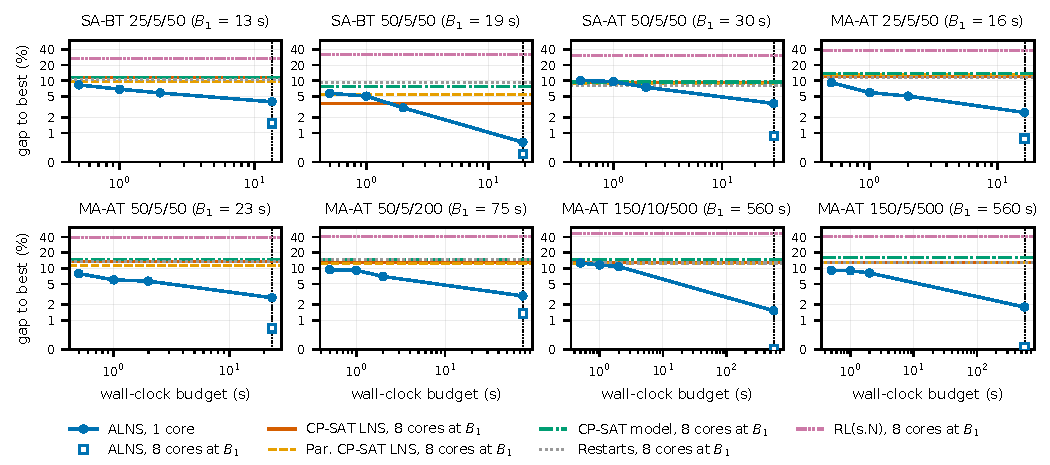
\includegraphics[width=\textwidth]{figures/budget}
\caption{Mean gap to the best known plan (\%, symmetric log scale) against the wall-clock budget. ALNS on one core
(line) at 0.5, 1, 2\,s and $B_1$, and on 8 cores at $B_1$ (open square), against every competitor on 8 cores at $B_1$
(horizontal lines; the dotted vertical line marks $B_1$). CTAS-D, which fails on most instances, is not shown. Test
instances, 50 per setting.}
\label{fig:budget}
\end{figure*}

\paragraph{C1: equal compute.} ALNS on 8 cores is better than every competitor at the same budget $B_1$ on
\ConeBheld{} of the \ConeBsettings{} settings (Table~\ref{tab:ratios}a): \ConeBsig{} of the \ConeBtests{} tests are
significant after Holm's correction (largest adjusted $p = \ConeBmaxp$), and ALNS gives the shorter plan in
\ConeBwon{} of the \ConeBpairs{} paired runs. Its plans are \ConeBclasslo--\ConeBclasshi\% shorter than those of the
three CP-SAT-based methods and greedy restarts, and \ConeBrlgainlo--\ConeBrlgainhi\% shorter than those of the RL
policy.
Settings where C1 does not hold: \ConeBfaillist. The pre-registered decision rule (C1 on at least six of the eight
settings) therefore \ConeBverdict. With twice the budget, $2B_1$, ALNS stays ahead of parallel CP-LNS, CP-SAT full
model and greedy restarts in \ConeBBheld{} of \ConeBBsettings{} settings (\ConeBBsig{} of \ConeBBtests{} tests
significant, plans \ConeBBclasslo--\ConeBBclasshi\% shorter).

\begin{table}[t]
\centering
\small
\caption{Mean gap to the best plan found by any run (\%) and CPU used (CPU seconds of all processes and threads, as a share of 8 cores for $B_1$); range over the eight settings. Every method runs on 8 cores at $B_1$, except ALNS on 1 core for 2\,s. CTAS-D: share of the instances solved within $B_1$, up to 200 tasks.}
\label{tab:methods}
\begin{tabular}{lcc}
\toprule
Method & Gap to best (\%) & CPU used (\%) \\
\midrule
ALNS, 8 cores & 0.0--0.9 & 98--100 \\
ALNS, 1 core, 2\,s & 2.6--10.1 & 0.04--1.7 \\
\midrule
CP-LNS & 3.9--13.8 & 34--79 \\
Parallel CP-LNS & 4.9--13.3 & 97--101 \\
CP-SAT full model & 5.8--16.3 & 51--90 \\
CTAS-D (exact MILP) & solves 0--98\% & 49--96 \\
Greedy restarts & 6.5--14.4 & 97--100 \\
RL policy (published) & 28.3--63.6 & 89--97 \\
\bottomrule
\end{tabular}
\end{table}


\paragraph{Parallelism does not rescue CP-SAT.} CP-LNS uses only \Cpucpsatlo--\Cpucpsathi{} of its 8 cores
(Table~\ref{tab:methods}), because building each subproblem is serial between the multi-threaded solver calls.
Parallel CP-LNS keeps all cores busy (\Cpupcpsatlo--\Cpupcpsathi) and makes many more solver calls
(Table~\ref{tab:steps}), but it is not clearly better: the ratio ALNS / competitor is \ConeBpcpsatlo--\ConeBpcpsathi{}
against the parallel version and \ConeBcpsatlo--\ConeBcpsathi{} against the single search. CP-SAT's own search on the
full model does no better (\ConeBcpfulllo--\ConeBcpfullhi): on the larger instances it rarely improves on the greedy
plan it starts from (in tuning, it ended with that plan on 13 of 16 instances with 200 or 500 tasks). Shorter solver
calls do not help either: with 200 tasks, calls of 0.5\,s or less spent their time building and presolving the
subproblem and never improved the plan in our tuning runs.

\paragraph{The exact MILP.} CTAS-D finds a plan within $B_1$ for \CtasSolved{} of the \CtasRuns{} test instances with
up to 200 tasks (Table~\ref{tab:ratios}a). This matches the published picture, where Gurobi solved few instances of most
50-task settings within an hour \cite{dai2025heterogeneous}: the MILP is a strong method on 20 tasks, where our port
beats the shipped Gurobi solutions, but not a competitor at this scale.

\paragraph{The learned policy.} The RL policy ends \Gaprllo--\Gaprlhi\% above the best known plans, although it
completes \RLNlo{} to \RLNhi{} times the published number of rollouts. Greedy restarts alone give plans
\RestartsRLlo--\RestartsRLhi\% shorter (ratio of means): a careful construction with restarts already closes much of
the gap to the learned policy, and search closes the rest.

\paragraph{C2: one core.} ALNS on a single core for 2\,s is significantly better than every competitor on 8 cores at
$B_1$ on \Ctwoheld{} of the \Ctwosettings{} settings: \Ctwoheldlist{} (Table~\ref{tab:ratios}b;
\Ctwosig{} of \Ctwotests{} tests significant). It does not hold on \Ctwofaillist. Against the learned policy it holds
everywhere, with plans \Ctworlgainlo--\Ctworlgainhi\% shorter than those the RL policy finds on 8 cores in 7 to 280
times the wall-clock time. At 1\,s and 0.5\,s, C2 holds on \CtwoOneheld{} and \CtwoHalfheld{} settings, and at $B_1$
ALNS on one core has a lower mean gap than every 8-core competitor on \OneCoreBoneAhead{} settings (descriptive;
Figure~\ref{fig:budget}).

\paragraph{Scaling with cores.} Eight workers instead of one improve ALNS at $B_1$ by only
\Workersgainlo--\Workersgainhi\% (ratio \Workerslo--\Workershi). Most of its advantage is thus per-core efficiency,
not parallelism.

\paragraph{How good are the plans?} The best known plans on 50 or more tasks come from ALNS runs, which raises the
question whether ALNS is merely close to itself. On the validation instances we ran parallel CP-LNS and CP-SAT full
model for 300\,s on 8 cores, starting from greedy plans only, with 10 to 20 times the compute of $B_1$. On none of the
\RefValInstances{} validation instances with 50 or more tasks did any run without an ALNS component match the best
ALNS-derived plan; the best of them is on average \RefValFreelo--\RefValFreehi\% longer per setting, while ALNS on 8
cores at $B_1$ ends \Gapalnslo--\Gapalnshi\% above the best known plans on the test instances. The certified lower bounds of CP-SAT remain
\RefValBoundlo--\RefValBoundhi\% below the best known plans, so the distance to the optimum is unknown; the paired
ratios above do not depend on it.

\paragraph{Execution.} All \RunsBone{} runs on 8 cores at $B_1$ were scored; \LateBone{} of them overran their budget
by more than 10\% + 0.25\,s and were scored at the budget as pre-registered: \LateRL{} runs of the RL policy, whose
last batch of rollouts can end after the deadline and which keeps no intermediate plan, so that such a run counts as a
failure, \LateALNS{} of ALNS and \LateOther{} of the other competitors. If every late run is instead scored by the
final plan it returned (descriptive, not pre-registered), ALNS's plans are \Sensrlgainlo--\Sensrlgainhi\% shorter
than those of the RL policy. Jobs with more than 40\% throttled CPU periods were re-run and left out; the per-row host conditions are
in the supplement.

\section{Discussion}
\label{sec:discussion}

\paragraph{Why search wins here.} The learned policy builds a plan in one pass of sequential decisions, and sampling
more rollouts adds diversity but no improvement of a given plan. ALNS spends the same time improving one plan with
many cheap, exact moves: our representation keeps every move feasible, and Eq.~\eqref{eq:insert} scores an insertion
in time linear in the coalition size, so a single core evaluates thousands of neighbours per second. The CP-SAT
baselines search a richer neighbourhood per step but pay for building and solving a model at every step, which is why
parallelising them helps little.

\paragraph{Implications.} We do not claim that learning is the wrong tool for multi-robot coordination: a
decentralised policy can react to events that a central plan cannot. But the static planning performance of
learned policies should be measured against strong search at matched compute, on the same cores and with the CPU
use reported. The published comparison missed plans \ConeBrlgainlo--\ConeBrlgainhi\% shorter, which a standard
operations-research technique adapted to coalitions finds at the same budget, and largely already on one core in 2\,s.

\paragraph{Limitations.}
\begin{itemize}
\item \emph{Static, centralised planning.} We evaluate plans for fully known, static instances, as the benchmark
  does. The RL policy is decentralised and reactive, which matters under uncertainty and with dynamic arrivals; we
  did not evaluate such settings in the confirmatory run. An exploratory dynamic variant did not pass the go/no-go
  gates we had set on dev, and it is reported in the supplement as a negative result.
\item \emph{One benchmark.} All instances come from one generator with Euclidean travel, one speed and a makespan
  objective. We expect the representation to transfer to other objectives and travel models, but have not tested it.
\item \emph{RL on CPU.} To match compute, the policy runs on the same CPU cores as every other method. On a GPU it
  could draw more rollouts. It already draws \RLNlo{} to \RLNhi{} times the published number, which makes its plans
  only \RLsamplegainlo--\RLsamplegainhi\% shorter than with ten rollouts.
\item \emph{Unknown optimality gaps.} On 50 or more tasks no method proves optimality, and the certified bounds are
  loose, so we report gaps to the best known plans and ratios between methods.
\item \emph{Tuning.} ALNS was developed and tuned on the dev split of the same generator. Every competitor with a
  parameter was tuned per setting on the same split, which favours the competitors.
\item \emph{Pre-registration.} The val dry run was known before the freeze, the test-split results of the
  constructor and of the RL policy had been seen in an earlier phase, and the released test set of the benchmark
  (not blind) was used to choose CTAS-D's solver. No ALNS or CP-SAT variant and no CTAS-D port ran on the test split
  before the freeze.
\item \emph{Single host and seed.} All timed runs used one host and one seed per instance, method and budget. On
  val, 52 cells measured on two different hosts agreed within 2\%.
\item \emph{CTAS-D.} Our port solves the published model with an open solver on a time grid of $10^{-3}$ and counts
  model building in the budget; it is not the benchmark paper's Gurobi run, although it beats that run on the
  released 20-task instances.
\end{itemize}

\section{Conclusion}
\label{sec:conclusion}

On the HeteroMRTA benchmark, an adaptive large neighbourhood search over a deadlock-free coalition representation
with exact linear-time insertion finds plans \ConeBrlgainlo--\ConeBrlgainhi\% shorter than the published
reinforcement-learning policy and \ConeBclasslo--\ConeBclasshi\% shorter than three CP-SAT baselines and restarts, while
the exact MILP rarely finds a plan at all, at equal compute and under a pre-registered protocol. We release the solver, the harness, the pre-registration and every result row, so that future learned
planners can be compared against this baseline at matched budgets.


\section*{Use of AI Assistance}
% USER: this statement must be accurate and is the authors' responsibility (AAMAS 2027 AI policy). Check the tool
% versions, the share of the work done with the assistant and the wording before submission; the AAMAS policy permits
% AI for polishing and formatting text and for code, and requires details (tool, version, prompts) where AI helped to
% create hypotheses or methodology, including experimental design.
This work used an AI coding assistant, Claude Code (Anthropic, version 2.1) with Anthropic's Claude models (including
Claude Opus 5.5). Under the authors' direction it wrote most of the code of the solver, the competitors and the
experiment harness; it proposed and critiqued parts of the experimental design, the analysis plan and the
pre-registration, which the authors reviewed, changed where needed and approved before the confirmatory run; and it
drafted and polished parts of the text. Figure~\ref{fig:overview} was drawn as TikZ code by the assistant; as layout
references it used draft images from an image-generation tool (OpenAI Codex CLI), which are not part of the paper or
the supplementary material. The data figures are plotted from the result files by our scripts. The authors checked the code with tests against the benchmark's simulator,
with the reproduction of the published results of the learned policy and of CTAS-D, and with independent reference
solutions; every citation was checked against its publisher or index record. The supplementary material lists the
tool versions and the prompts used for the experimental design. The authors take full responsibility for the content
of this paper.


\balance
\bibliographystyle{ACM-Reference-Format}
\bibliography{refs}

\end{document}
